\taskpic{Массивная доска AB скользит со скоростью $u$ по гладкой
  горизонтальной поверхности. Из точки С той же поверхности
  одновременно вылетают две легкие шайбы. Первая шайба скользит по
  поверхности в направлении $CC_1$ параллельно доске АВ со скоростью
  $v_1$, вторая скользит со скоростью $v_2$ под углом $\alpha$ к
  $CC_1$. Через некоторое время шайбы сталкиваются в точке
  D. Определите скорости шайб $v_1$ и $v_2$ до столкновения, если
  известно, что время от начала движения шайб до их столкновения в $n$
  раз превышает время от начала движения шайб до столкновения второй
  шайбы с доской. При ударе шайбы о доску потерь энергии не
  происходит.}{
  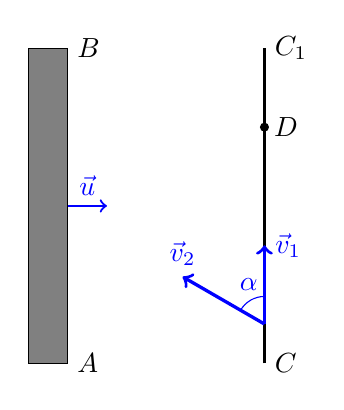
\begin{tikzpicture}
    \draw[fill=gray] (0,0) rectangle (0.5,4);
    \draw (0.5,0) node[right] {$A$};
    \draw (0.5,4) node[right] {$B$};
    \draw[thick,blue,->] (0.5,2) -- (1,2) node[midway,above]
    {$\vec{u}$};
    \draw[thick] (3,0) node[right] {$C$} -- (3,4) node[right] {$C_1$};
    \draw[very thick,->,blue] (3,0.5) -- (3,1.5) node[right]
    {$\vec{v}_1$};
    \draw[very thick,->,blue] (3,0.5) -- ++(150:1.2cm) node[above]
    {$\vec{v}_2$};
    \draw[blue] (3,0.85) arc (90:150:0.35cm);
    \draw (2.8,1) node[blue] {$\alpha$};
    \draw[fill=black] (3,3) circle (0.05cm) node[right] {$D$};
  \end{tikzpicture}
}
